\documentclass[aspectratio=169,11pt]{beamer}
\usepackage[utf8]{inputenc}
\usepackage[T1]{fontenc}
\usepackage{amsmath,amssymb,mathtools}
\usepackage{tikz}
%\usetheme{Madrid}
\usecolortheme{default}
\setbeamertemplate{navigation symbols}{}
\setbeamertemplate{theorems}[numbered]
\uselanguage{Portuguese}
\languagepath{Portuguese}
\providecommand{\proofname}{Prova}
\newtheorem{proposition}{Proposição}

\newcommand{\E}{\mathbb{E}}
\newcommand{\PP}{\mathbb P}
\newcommand{\Var}{\operatorname{Var}}
\newcommand{\Ind}[1]{\mathbf{1}_{#1}}
\newcommand{\conj}[1]{\{#1\}}
\newcommand{\card}[1]{\lvert #1\rvert}
\newcommand{\tq}{\colon}

\title[Hashing]{Hashing: funções aleatórias e colisões}

\author{J. D.}
\institute{UFABC}
\date{\today}

\begin{document}

%% ---------------------------------------------------------------- 1
\begin{frame}
  \titlepage
\end{frame}

%% ---------------------------------------------------------------- 2
\begin{frame}{Roteiro }
  \begin{enumerate}
  \item[1.] \textbf{Funções de hash} e por que precisamos de aleatoriedade 
  \item[2.] \textbf{Tabelas de espalhamento} e custo de busca com função aleatória 
  \item[3.] \textbf{A maior lista}: cota $O(\log n/\log\log n)$
  \item[4.] \textbf{Paradoxo dos aniversários} e o limiar $\sqrt n$ 
  \item[5.] \textbf{Variância} e independência par a par 
  \item[6.] \textbf{Síntese}: o que basta para famílias universais
  \end{enumerate}
  \vspace{1em}
  \begin{alertblock}{Fio condutor}
    Uma função totalmente aleatória espalha bem, mas não tem descrição curta. \\
    Quais propriedades dela \emph{realmente} usamos?
  \end{alertblock}
\end{frame}

%% ================================================================ 1
\section{Funções de hash}

%% ---------------------------------------------------------------- 3
\begin{frame}{O que é uma função de hash?}
  \begin{definition}
    Uma \alert{função de hash} é uma função $h\tq U\to N$, onde o universo $U$
    é \emph{muito grande} e $N=\conj{0,1,\dots,n-1}$.
  \end{definition}
  \begin{itemize}
  \item $h(x)$ é um ``resumo'' de $x$: ocupa pouco espaço, é comparável e
    serve de índice em tempo constante.
  \item Como $\card U\gg\card N$, há \alert{colisões}: $x\neq y$ com
    $h(x)=h(y)$. Pelo princípio da casa dos pombos, não dá para evitá-las.
  \end{itemize}
  \pause
  \vspace{0.5em}
  \textbf{Usos:} dicionários (tabelas de espalhamento), impressões digitais e
  verificação de igualdade, desaleatorização, criptografia (exige mais:
  colisões difíceis de achar).
  \begin{block}{Foco desta aula}
    Propriedades \emph{probabilísticas} de famílias de funções.
  \end{block}
\end{frame}

%% ---------------------------------------------------------------- 4
\begin{frame}{O que torna uma função de hash útil?}
  Não é ser injetora. São propriedades que dependem do uso:
  \begin{itemize}
  \item[\textbf{(i)}] \textbf{fácil de computar}: $h(x)$ em tempo (quase) constante;
  \item[\textbf{(ii)}] \textbf{descrição curta}: poucos bits para armazenar $h$;
  \item[\textbf{(iii)}] \textbf{espalhar bem} os elementos de um conjunto $S\subseteq U$:
    valores $h(x)$, $x\in S$, aproximadamente uniformes em $N$, poucas colisões.
  \end{itemize}
  \pause
  \vspace{0.5em}
  \begin{alertblock}{O problema com (iii)}
    Para \emph{qualquer} $h$ fixa, existe $S$ em que todos colidem:
    basta escolher $m \coloneqq |S|$ elementos numa mesma pré-imagem
    (tem tamanho $\ge\card U/n$).  Nenhuma $h$ determinística espalha
    bem \emph{todos} os conjuntos.
  \end{alertblock}
  \pause
  \textbf{Saída:} sortear $h$ de uma família $\mathcal H$ e analisar o
  comportamento \emph{esperado}, ou com alta probabilidade, para qualquer $S$
  \emph{fixo}.
\end{frame}

%% ================================================================ 2
\section{Tabelas de espalhamento}

%% ---------------------------------------------------------------- 5
\begin{frame}{Tabela de espalhamento (com listas ligadas)}
  \begin{columns}[T]
    \begin{column}{0.48\textwidth}
      \begin{itemize}
      \item Vetor $H$ com $n$ posições; cada $H[i]$ é uma lista ligada.
      \item Acesso via $h\tq U\to\conj{0,1,\dots,n-1}$: o elemento $x$ vive na
        lista $H[h(x)]$.
      \item $S\subseteq U$ com $m=\card S$; interessa o caso $m=\Omega(n)$.
      \item Um vetor de bits de tamanho $\card U$ daria busca $O(1)$, mas é
        inviável.
      \end{itemize}
    \end{column}
    \begin{column}{0.5\textwidth}
      \centering
      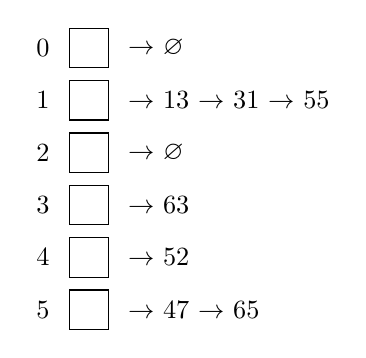
\begin{tikzpicture}[cell/.style={draw,minimum height=1.5em,minimum width=1.5em,inner sep=0pt}, scale=0.95, transform shape]
        \foreach \i/\t in {0/{$\varnothing$},1/{13 $\to$ 31 $\to$ 55},2/{$\varnothing$},3/{63},4/{52},5/{47 $\to$ 65}} {
          \node[left] at (0,-\i*0.7) {\i};
          \node[cell] at (0.4,-\i*0.7) {};
          \node[right,anchor=west] at (0.8,-\i*0.7) {$\to$ \t};
        }
      \end{tikzpicture}

      {\small $S=\{13,31,47,52,55,63,65\}$, $h(x)=x \bmod 6$}
    \end{column}
  \end{columns}
\end{frame}

%% ---------------------------------------------------------------- 6
\begin{frame}{Operações e custos}
  \begin{description}
  \item[Inserção] colocar $x$ no início de $H[h(x)]$: custo \alert{constante}.
  \item[Remoção] (com apontador para $x$) retirar da lista: custo constante.
  \item[Busca] percorrer a lista $H[h(x)]$. Pode ser \emph{com sucesso}
    ($x\in S$) ou \emph{sem sucesso} ($x\notin S$).
  \end{description}
  \pause
  \begin{block}{Quem manda no desempenho?}
    O pior caso da busca é o tamanho da \alert{maior lista}. Tudo se reduz a
    entender os tamanhos das listas, que dependem de como $h$ distribui $S$.
  \end{block}
  \pause
  \textbf{Primeiro modelo:} $h$ uniforme em $N^U$ (todas as $n^{\card U}$
  funções). Equivale a sortear, \emph{independentemente} para cada $x\in U$,
  um valor $h(x)$ uniforme em $N$.
\end{frame}

%% ---------------------------------------------------------------- 7
\begin{frame}{Função aleatória: probabilidade de colisão e carga}
  Para todo $x\in U$ e $i\in N$: \quad $\PP[h(x)=i]=\dfrac1n$.
  \pause
  \begin{block}{Colisão de um par}
    Para $x\neq y$, por independência,
    \[
      \PP[h(x)=h(y)]=\sum_{i\in N}\PP[h(x)=i]\,\PP[h(y)=i]
      = n\cdot\frac1n\cdot\frac1n=\frac1n .
    \]
  \end{block}
  \pause
  \begin{definition}
    A \alert{carga} da tabela é $c=m/n$, o número esperado de elementos de $S$
    por posição.
  \end{definition}
  \vspace{-0.3em}
  Sobre $c$: se $m=\Theta(n)$, então $c=\Theta(1)$.
\end{frame}

%% ---------------------------------------------------------------- 8
\begin{frame}{Tamanho esperado da lista $H[h(x)]$}
  O número de itens na lista de $x$ é $\sum_{y\in S}\Ind{[h(x)=h(y)]}$, e
  \[
    \E\,\Ind{[h(x)=h(y)]}=
    \begin{cases}
      1/n, & y\neq x,\\
      1, & y=x.
    \end{cases}
  \]
  \pause
  Pela \alert{linearidade da esperança},
  \[
    \E\,\bigl|H[h(x)]\bigr|=
    \begin{cases}
      \dfrac mn=c, & x\notin S,\\[2ex]
      \dfrac{m-1}{n}+1, & x\in S.
    \end{cases}
  \]
  \pause
  \begin{alertblock}{Conclusão}
    Com $h$ aleatória em $N^U$, o tempo esperado de busca é proporcional à
    carga: \alert{$O(1)$ quando $n=\Theta(m)$}.
  \end{alertblock}
\end{frame}

%% ---------------------------------------------------------------- 9
\begin{frame}{Custo esperado das buscas}
  \begin{proposition}
    Seja $H$ com $n$ posições e $h$ aleatória; elementos inseridos no início
    das listas. Então
    \begin{enumerate}
    \item busca \emph{sem sucesso}: tempo esperado $c+1$;
    \item busca \emph{com sucesso}: tempo esperado $1+\dfrac c2-\dfrac1{2n}$.
    \end{enumerate}
  \end{proposition}
  \pause
  \textbf{Ideia da prova do item 2.} Se $x$ foi o $i$-ésimo inserido, só os
  $m-i$ elementos inseridos \emph{depois} podem ficar na frente de $x$; em
  média $(m-i)/n$ deles colidem com $x$. Logo
  \[
    \frac1m\sum_{i=1}^m\Bigl(1+\frac{m-i}n\Bigr)=1+\frac{m-1}{2n}
    =1+\frac c2-\frac1{2n}.
  \]
\end{frame}

%% ---------------------------------------------------------------- 10
\begin{frame}{Qual é o problema?}
  \begin{columns}[T]
    \begin{column}{0.5\textwidth}
      \textbf{O que ganhamos}
      \begin{itemize}
      \item busca esperada $O(1)$;
      \item maior lista $O(\log m)$ com alta probabilidade (próximo bloco).
      \end{itemize}
    \end{column}
    \begin{column}{0.5\textwidth}
      \textbf{O que perdemos}
      \begin{itemize}
      \item uma função aleatória em $N^U$ precisa de $\approx\card U\log n$ bits
        para ser descrita;
      \item guardar $h$ custa mais que o vetor de bits que queríamos evitar.
      \end{itemize}
    \end{column}
  \end{columns}
  \vspace{1.2em}
  \pause
  \begin{block}{Pergunta}
    Das propriedades que usamos até aqui, quais dependem de $h$ ser
    \emph{totalmente aleatória.}
\end{block}
  Vamos acompanhar isso ao longo das próximas análises.
\end{frame}

%% ================================================================ 3
\section{A maior lista}

%% ---------------------------------------------------------------- 11
\begin{frame}{A maior lista é sublogarítmica}
  \begin{lemma}
    Seja $X_i=\card{\conj{y\in S\tq h(y)=i}}$, $c\le1$ e $n$ suficientemente
    grande. Então
    \[
      \PP\Bigl[\max_i X_i\ \ge\ \frac{8\ln n}{\ln\ln n}\Bigr]\ \le\ \frac1n .
    \]
  \end{lemma}
  Como $n=\Theta(m)$, a maior lista tem tamanho $O(\log m/\log\log m)$ com
  probabilidade $\ge1-1/n$.
  \pause
  \begin{block}{Estratégia}
    \begin{enumerate}
    \item cota para $\PP[X_i\ge k]$ por união sobre subconjuntos $T\subseteq S$;
    \item limitar $k!$ por baixo;
    \item cota da união sobre as $n$ posições e escolha de $k$.
    \end{enumerate}
  \end{block}
\end{frame}

%% ---------------------------------------------------------------- 12
\begin{frame}{Prova (1): cota para uma posição}
  Se $X_i\ge k$, existe $T\subseteq S$, $\card T=k$, com $h(y)=i$ para todo
  $y\in T$. Pela independência, cada $T$ tem probabilidade $n^{-k}$. Pela
  cota da união,
  \[
    \PP[X_i\ge k]\le\binom mk\frac1{n^k}\le\frac{m^k}{k!\,n^k}
    =\frac{c^k}{k!}\le\frac1{k!}.
  \]
  \pause
  De $e^k=\sum_{j\ge0}k^j/j!\ge k^k/k!$ obtemos $k!\ge(k/e)^k$, logo
  \[
    \PP[X_i\ge k]\le\Bigl(\frac ek\Bigr)^k.
  \]
  \pause
  Cota da união sobre as $n$ listas (\emph{não} precisamos que sejam
  independentes):
  \[
    \PP\bigl[\max_iX_i\ge k\bigr]\le n\Bigl(\frac ek\Bigr)^k
    =n\,e^{-k(\ln k-1)}.
  \]
\end{frame}

%% ---------------------------------------------------------------- 13
\begin{frame}{Prova (2): escolha de $k$}
  Tome $k_0=\dfrac{8\ln n}{\ln\ln n}$, $k=\lceil k_0\rceil$,
  $y=\ln\ln n$ e $\phi(t)=t(\ln t-1)$, crescente para $t\ge1$.
  \pause
  \begin{itemize}
  \item $\ln k_0=\ln8+y-\ln y\ \ge\ \tfrac12y$ (pois $\ln y\le\tfrac y2+\ln8$ para todo $y>0$);
  \item para $n$ grande, $y\ge4$, então $\ln k_0-1\ge\tfrac12y-1\ge\tfrac14y$.
  \end{itemize}
  \pause
  Logo
  \[
    \phi(k)\ge\phi(k_0)=k_0(\ln k_0-1)\ge\frac{8\ln n}{y}\cdot\frac y4=2\ln n,
  \]
  e portanto
  \[
    \PP\bigl[\max_iX_i\ge k\bigr]\le n\,e^{-\phi(k)}\le n\,e^{-2\ln n}=\frac1n.
    \qquad\blacksquare
  \]
\end{frame}

%% ---------------------------------------------------------------- 14
\begin{frame}{Observações sobre a cota}
  \begin{itemize}
  \item \textbf{Carga constante.} Se $c\le C$, a cota vira $(Ce/k)^k$; basta
    trocar $e$ por $Ce$ e ajustar a constante $8$.
    \pause
  \item \textbf{A cota é justa.} Um argumento de segundo momento sobre o
    número de listas com $\ge k$ elementos mostra que, com alta probabilidade,
    a maior lista tem tamanho $\Omega(\log n/\log\log n)$. Portanto
    \[
      \max_iX_i=\Theta\Bigl(\frac{\log n}{\log\log n}\Bigr).
    \]
    \pause
  \item \textbf{O que foi usado?} A independência de $k$ valores $h(y)$ ao
    mesmo tempo (probabilidade $n^{-k}$ para cada $T$).
  \end{itemize}
  \begin{alertblock}{Guardem isto}
    Este resultado precisa de independência de \emph{muitas} variáveis. Será
    o preço da descrição curta nas famílias universais.
  \end{alertblock}
\end{frame}

%% ================================================================ 4
\section{Paradoxo dos aniversários}

%% ---------------------------------------------------------------- 15
\begin{frame}{Número esperado de colisões}
  Seja $C$ o número de pares $\{x,y\}\subseteq S$ que colidem:
  $C=\sum_{\{x,y\}}\Ind{[h(x)=h(y)]}$. Por linearidade,
  \[
    \E\,C=\binom m2\frac1n=\frac{m(m-1)}{2n}.
  \]
  \pause
  Pela desigualdade de Markov,
  \[
    \PP[C=0]\ \ge\ 1-\E\,C=1-\frac{m(m-1)}{2n}.
  \]
  Em particular, para $m=\sqrt n$: $\E\,C<\tfrac12$ e $\PP[C=0]\ge\tfrac12$.
  \pause
  \begin{block}{Observação}
    Só usamos $\PP[h(x)=h(y)]=1/n$ para pares. Isto é \alert{informação sobre
    pares}.
  \end{block}
\end{frame}

%% ---------------------------------------------------------------- 16
\begin{frame}{Probabilidade de nenhuma colisão}
  Para $m\le n$ há $n(n-1)\cdots(n-m+1)$ sequências sem repetição em $N^m$:
  \begin{align*}
    \PP[C=0]&=\prod_{j=1}^{m-1}\Bigl(1-\frac jn\Bigr)
    \;<\;\prod_{j=1}^{m-1}e^{-j/n}
    =\exp\Bigl(-\frac{m(m-1)}{2n}\Bigr),
  \end{align*}
  usando $1-x<e^{-x}$.
  \pause
  \vspace{0.5em}
  \begin{exampleblock}{Paradoxo dos aniversários ($m=23$, $n=365$)}
    \[
      \PP[C>0]>1-e^{-506/730}>\tfrac12,
    \]
    pois $506/730\approx0{,}693151>\ln2\approx0{,}693147$. Basta uma turma de
    23 pessoas para haver aniversário repetido com probabilidade $>1/2$.
  \end{exampleblock}
\end{frame}

%% ---------------------------------------------------------------- 17
\begin{frame}{O limiar $\sqrt n$}
  \textbf{Cota inferior.} Para $x\in(0,3/4]$, $1-x>e^{-2x}$. Se $m\le\tfrac34n$,
  \[
    \PP[C=0]>\prod_{j=1}^{m-1}e^{-2j/n}=\exp\Bigl(-\frac{m(m-1)}n\Bigr).
  \]
  \pause
  \begin{itemize}
  \item Se $m\le\sqrt n$: $\PP[C=0]>e^{-1}>0{,}36$ (limitada por constante positiva).
  \item Se $m=\omega(\sqrt n)$: a cota superior $e^{-m(m-1)/(2n)}\to0$.
  \end{itemize}
  \pause
  \begin{alertblock}{Limiar}
    $\sqrt n$ é o limiar para o aparecimento de colisões.
  \end{alertblock}
  \begin{small}
  Markov dá $\PP[C=0]\ge1-\E C>\tfrac12$ para $m\le\sqrt n$, melhor que $e^{-1}$
  nesse regime, mas vira trivial para $m\ge\sqrt{2n}+1$ (onde $\E C\ge1$). A
  cota exponencial vale até $m\le\tfrac34n$.
  \end{small}
\end{frame}

%% ================================================================ 5
\section{Variância e independência par a par}

%% ---------------------------------------------------------------- 18
\begin{frame}{Variância do tamanho de uma lista}
  Seja $X_i=\sum_{x\in S}\Ind{[h(x)=i]}$, com $\E X_i=c$. Para $x\neq y$ os
  indicadores são independentes. Então
  \[
    \Var X_i=\sum_{x\in S}\frac1n\Bigl(1-\frac1n\Bigr)
    =c\Bigl(1-\frac1n\Bigr).
  \]
  \pause
  Chebyshev:
  \[
    \PP[\,|X_i-c|\ge t\,]\le\frac{c(1-1/n)}{t^2}\le\frac c{t^2}.
  \]
  \pause
  Com $t=c$: $\PP[X_i\ge2c]\le\frac1c$, só útil para $c$ grande.
  \vspace{0.5em}
  \begin{block}{Observação-chave}
    Esta conta só usa que os indicadores $\Ind{[h(x)=i]}$ são independentes
    \alert{dois a dois}.
  \end{block}
\end{frame}

%% ---------------------------------------------------------------- 19
\begin{frame}{Maior lista via Chebyshev}
  Cota da união sobre as $n$ listas:
  \[
    \PP\bigl[\max_iX_i\ge c+t\bigr]\le n\cdot\frac c{t^2}=\frac m{t^2}.
  \]
  Com $t=\sqrt{2m}$, a maior lista tem tamanho
  \[
    \le c+\sqrt{2m}=O(\sqrt m)
  \]
  com probabilidade pelo menos $1/2$.
  \pause
  \begin{exampleblock}{Comparação}
    \begin{center}
    \begin{tabular}{lll}
      \textbf{Método} & \textbf{Cota} & \textbf{Independência usada} \\\hline
      Cota da união sobre $T$ & $O(\log n/\log\log n)$ & muitas variáveis \\
      Chebyshev & $O(\sqrt m)$ & só pares
    \end{tabular}
    \end{center}
  \end{exampleblock}
  \small Mais fraca, mas vale também para famílias com descrição curta.
\end{frame}

%% ---------------------------------------------------------------- 20
\begin{frame}{Variância do número de colisões}
  $C=\sum_{\{x,y\}}\Ind{[h(x)=h(y)]}$. Para pares distintos
  $\{x,y\}\neq\{z,w\}$:
  \begin{itemize}
  \item disjuntos: dependem de quatro valores independentes;
  \item com elemento comum ($\{x,y\}$ e $\{x,z\}$):
    \[
      \PP[h(x)=h(y)=h(z)]=\sum_{a\in N}\frac1{n^3}=\frac1{n^2}
      =\PP[h(x)=h(y)]\,\PP[h(x)=h(z)].
    \]
  \end{itemize}
  \pause
  Os indicadores são independentes dois a dois, logo
  $\Var C=\binom m2\bigl(\frac1n-\frac1{n^2}\bigr)$ e, por Chebyshev,
  \[
    \PP[C=0]\le\frac{\Var C}{(\E C)^2}=\frac{n(1-1/n)}{\binom m2}\approx\frac{2n}{m^2}.
  \]
  Para $m\gg\sqrt n$ há colisão com alta probabilidade, complementando o
  limiar do paradoxo dos aniversários.
\end{frame}

%% ---------------------------------------------------------------- 21
\begin{frame}{Cuidado: onde a independência de ordem maior entra}
  Na conta acima, a igualdade
  \[
    \PP[h(x)=h(y)=h(z)]=\PP[h(x)=h(y)]\,\PP[h(x)=h(z)]
  \]
  usa a independência de \alert{três} valores $h(x),h(y),h(z)$, e o caso de
  pares disjuntos usa \alert{quatro}.
  \pause
  \begin{alertblock}{Consequência}
    A fórmula para $\Var C$ vale para a função totalmente aleatória (e para
    famílias com independência de ordem $4$), mas \alert{não} para famílias
    apenas $2$-universais, para as quais só se garante $\E\,C=\binom m2/n$.
  \end{alertblock}
  \vspace{0.3em}
  Já a variância de $X_i$ usa apenas independência par a par.
\end{frame}

%% ================================================================ 6
\section{Síntese}

%% ---------------------------------------------------------------- 22
\begin{frame}{O que usamos de cada propriedade}
  \begin{center}
  \renewcommand{\arraystretch}{1.3}
  \begin{tabular}{lc}
    \textbf{Resultado} & \textbf{Propriedade necessária} \\\hline
    $\E\,C=\binom m2/n$, tempo esperado de busca & $\PP[h(x)=h(y)]\le1/n$ (pares) \\
    $\Var X_i$, maior lista $O(\sqrt m)$ & independência par a par \\
    $\Var C$ & independência de ordem $4$ \\
    maior lista $\Theta(\log n/\log\log n)$ & independência de muitas variáveis
  \end{tabular}
  \end{center}
  \pause
  \begin{block}{Ideia central}
    Qualquer família em que dois elementos distintos colidem com probabilidade
    $\le1/n$ tem, no máximo, o mesmo número esperado de colisões que uma
    função aleatória.
  \end{block}
\end{frame}

%% ---------------------------------------------------------------- 23
\begin{frame}{Para onde vamos: famílias universais}
  Funções aleatórias não são práticas: descrição de tamanho $\approx\card U$.
  \pause
  \begin{block}{A meta}
    Uma família $\mathcal H\subseteq N^U$ \emph{pequena} tal que, para
    $h\in\mathcal H$ uniforme,
    \[
      \PP_{h}[h(x)=h(y)]\le\frac1n\qquad\text{para todos }x\neq y\text{ em }U,
    \]
    com funções fáceis de computar e descrição curta.
  \end{block}
  \pause
  \begin{itemize}
  \item Comportar-se como função aleatória é propriedade da \emph{família},
    não de uma função isolada.
  \item Tudo que depende só de pares continuará valendo (esperança de
    colisões, tempo esperado de busca, $\Var X_i$).
  \end{itemize}
\end{frame}

%% ---------------------------------------------------------------- 24
\begin{frame}{Resumo}
  \begin{itemize}
  \item Colisões são inevitáveis; nenhuma $h$ fixa serve para todo $S$, então
    \alert{sorteamos $h$}.
  \item Com $h$ aleatória em $N^U$: busca esperada $O(1)$ para $n=\Theta(m)$.
  \item Maior lista: $\Theta(\log n/\log\log n)$ com alta probabilidade
    (cota da união + $k!\ge(k/e)^k$).
  \item Paradoxo dos aniversários: limiar de colisão em $m\approx\sqrt n$.
  \item Variância via Chebyshev precisa só de independência par a par; $\Var C$
    precisa de mais.
  \end{itemize}
  \vspace{0.5em}
  \begin{alertblock}{Próxima aula}
    Famílias universais e $2$-universais: descrição curta com garantias de
    pares.
  \end{alertblock}
\end{frame}

\end{document}

%%% Local Variables:
%%% mode: LaTeX
%%% TeX-master: t
%%% End:
